{\fontsize{12pt}{22pt} \textbf{Distribution functions}\par}

\vspace{5mm}

\underline{Mass function}

The probability mass function (p.m.f.) is the histogram of the distribution, that is:

- x-axis: values

- y-axis: frequency

\vspace{5mm}

\underline{Density function}

The probability density function (p.d.f.) is the "smoothed histogram" of the distribution.

\vspace{5mm}

\begin{center}
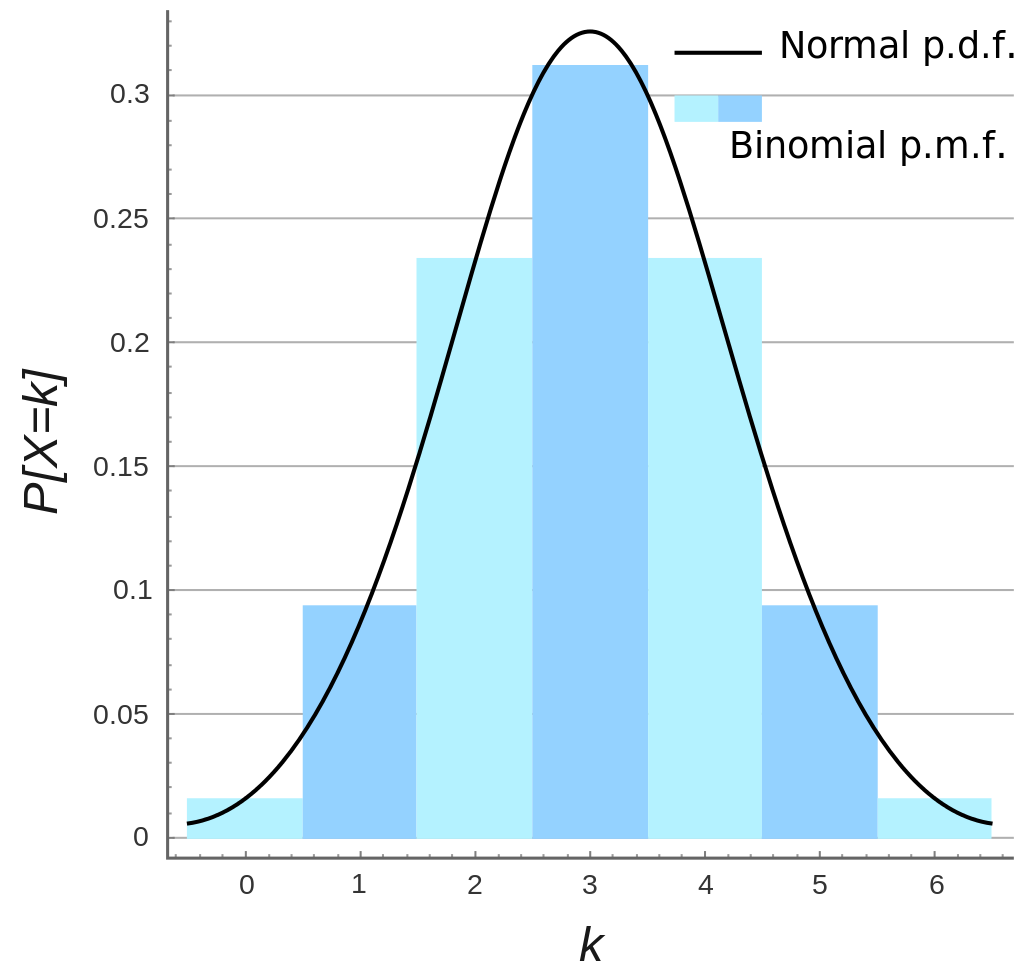
\includegraphics[scale=0.15]{mass_density_functions.png}
\end{center}

The major drawback of histograms is that they are not continuous, thus all points in the same range have the same estimated density. This can be adjusted in changing the bandwidth parameter (bins).

One of the common methods to solve this problem is the \textbf{Kernel Density Estimation} (KDE) method, also called the Parzen-Rosenblatt method. This method aims at estimating the density using the following formula:

$$\widehat f_n(x) = \frac{1}{nh} \sum_{i=1}^n K \Big( \frac{x-x_i}{h} \Big)$$

$x$ is any value that we want to plot the function on.

$x_i$ are the values from the distribution to be approximated.

$h$ is the bandwidth (or smoothing parameter). \\

Since Kernel functions usually have inputs in $\mathbb{R}^2$, $K \Big( \frac{x-x_i}{h} \Big)$ can also be written $K(\frac{x}{h}, \frac{x_i}{h})$.

We note that the KDE estimation is an average of kernels. Thus, if the choosen kernel is continuous, the estimated density is continuous.

Using the Gaussian kernel $K(x,y) = \frac{1}{\sqrt{2\pi}\sigma} \exp \bigg( {-\frac{||x-y||_2}{2 \sigma^2}} \bigg)$, we note that the estimated density is an average of generated gaussian distributions (kernel) that are centered in $x_i$. In the graph below (extracted from \href{https://github.com/savoga/various_projects/blob/master/Kernel_Density_Estimation.ipynb}{KDE notebook}), the distribution to be estimated is made of values $[1, 2.8, 3]$. Here the KDE method aims at building an average of three Gaussian distributions (\textit{gauss\_1}, \textit{gauss\_2}, \textit{gauss\_3}) centered respectively in 1, 2.8 and 3.

\begin{center}
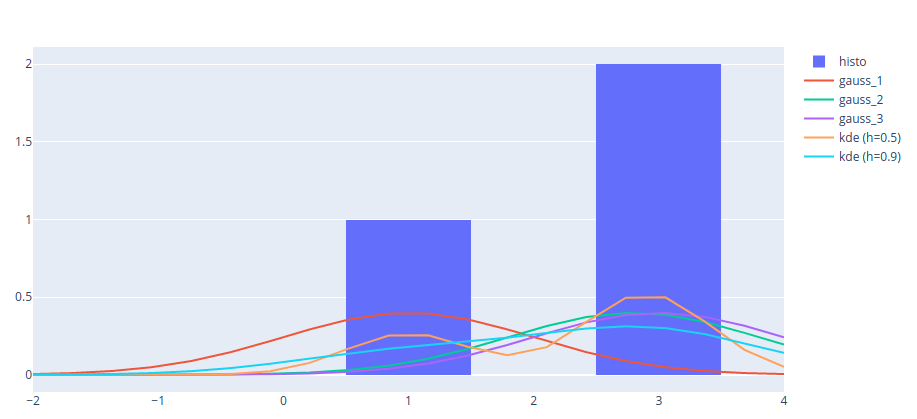
\includegraphics[scale=0.5]{KDE.png}
\end{center}

\vspace{5mm}

\underline{Cumulative distribution function}

The cumulative distribution function (c.d.f) is given by $F_X(x)= \mathbb{P}(X < x)$. 

The empirical distribution function is its estimation:
$\widehat{F}_n(x) = \frac{1}{n}\{\text{number of elements} < x\}$

\begin{center}
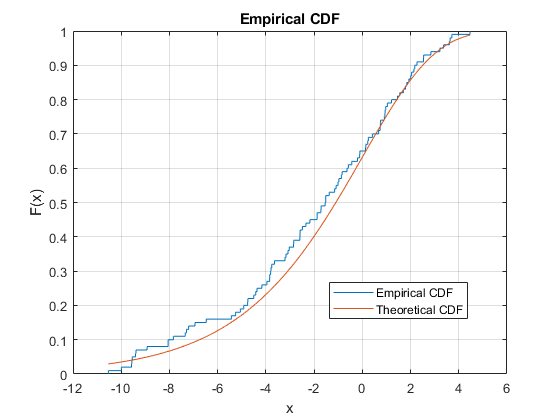
\includegraphics[scale=0.4]{CDF.png}
\end{center}

\lstset{language=Python}
\lstset{frame=lines}
\lstset{caption={Python CDF easy implementation}}
\lstset{label={lst:code_direct}}
\lstset{basicstyle=\footnotesize}
\begin{lstlisting}
plt.plot(np.sort(data_array), np.linspace(0, 1, len(data_array), endpoint=False))
\end{lstlisting}

\vspace{5mm}